\section{What the Operator Knows}\label{sec:reading}

A classical operator knows nothing about its offspring before they are
evaluated. We ask whether the LLM operator does: whether the outcome of
the child, and the algorithmic concepts it contains, are represented in
the model's state while it writes the code.

\subsection{The outcome of the child}
We fit linear probes (logistic or ridge regression) on the residual
stream of every layer at three positions: the last prompt token (before
the model writes), the mean over the prompt, and the mean over the
generated code. Each probe is compared with stacked baselines that use
what an AAD method could know without opening the model: search
metadata (operator, generation, parent fitness and outcome), the code
text (TF-IDF) and the model's output uncertainty (mean log-probability
and entropy of the generated tokens). Layers are selected inside nested
leave-one-run-out folds, and probes on shuffled labels stay at AUROC
$\le0.53$.

Figure~\ref{fig:probes} and Table~\ref{tab:incremental} summarise the
results. Whether the child will crash is decodable from the state
during writing with AUROC 0.85 (Qwen3-8B, layers 15--25), against 0.71
for the best single baseline and 0.77 for metadata and text combined;
the probe adds +0.08 (95\% CI 0.05 to 0.11) on top of both. Before the
model writes, at the last prompt token, the crash is barely predictable
(0.69): the failure arises while the code is written, not in the plan.
The same holds in Qwen3-14B (+0.06) and Gemma-3-12B (+0.02, with a
stronger text baseline). Whether the child will exceed its budget is
decodable with AUROC 0.93, but mostly because it is inherited: metadata
on the parent already reaches 0.91, and the probe adds only +0.03. The
parent's fitness is represented from the middle layers on (Spearman
$\rho\approx0.8$), but whether the child will improve on its parent, and
its fitness, are not decodable beyond metadata in any of the three
models (Appendix~\ref{app:reading}, Fig.~\ref{fig:probes-all}).

\begin{figure}[t]
  \centering
  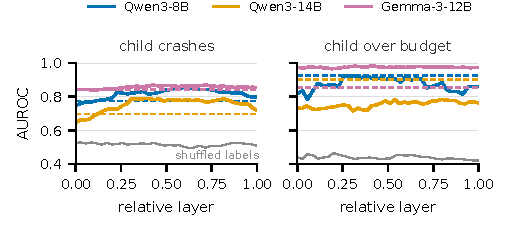
\includegraphics[width=\columnwidth]{figures/probes}
  \caption{Decodability of the child's outcome from the generator's
    state while it writes the code (mean over the generated tokens), per
    relative layer, three models. Dashed: metadata and code text
    combined, per model. Grey: Qwen3-8B probe on shuffled labels.}
  \Description{Two line plots of probe AUROC against relative layer.
    Left, crashes: the Qwen3-8B probe rises from 0.75 to 0.85 in the
    middle layers, above its baseline at 0.77; Qwen3-14B reaches 0.79
    against 0.70; Gemma-3-12B 0.87 against 0.84. Right, over budget: the
    probes reach 0.93 (Qwen3-8B) and 0.98 (Gemma) and the baselines are
    almost as high; the Qwen3-14B probe stays below its baseline.}
  \label{fig:probes}
\end{figure}

\subsection{Using what the model knows: a pre-screen}
A probe that predicts failure could save evaluations. We froze the
Qwen3-8B failure probe and a fixed threshold, and ran \llamea with a
pre-screen: a child whose score exceeds the threshold is not evaluated
and returns to the loop with a rejection message. After a power
analysis on 12 seeds, we pre-registered a non-inferiority test on the
best fitness of the run (margin 0.10 \aocc, one-sided paired $t$-test)
with 36 new seeds, each run once with and once without the screen.

On the new seeds the probe reaches AUROC 0.84--0.86; it flags 23.5\% of
the children and catches 69\% of the failures (Table~\ref{tab:prescreen}).
The screen skips 20.8\% of the evaluations. The best \aocc is 0.591 with
the screen and 0.628 without (difference $-0.037$, 90\% CI $-0.096$ to
$0.023$, $p=0.041$): non-inferior, narrowly, with no two-sided
difference (Wilcoxon $p=0.25$). Per-operator thresholds, a calibrated
risk and a running quantile do not beat the fixed threshold
(Table~\ref{tab:prescreen-rules}).

The probe's ranking also transfers to new problems without retraining.
On the Bragg and packing screens (Sec.~\ref{sec:steering}), the frozen
MA-BBOB probe reaches AUROC 0.77 and 0.72, close to probes refit on the
problem itself (0.84 and 0.73) and far above code length (0.55--0.57);
skipping its top 21\% would be 92\% and 79\% precise
(Table~\ref{tab:prescreen-transfer}). The threshold does not transfer,
since failure rates differ (70\% and 51\%), and must be recalibrated, for
instance as a fixed share of skipped children.

\paragraph{Is the pre-screen worth it?}
Skipped evaluations are not saved time, and the probe is not the only
cheap filter. We re-evaluated all 3,600 children of the unscreened runs
and timed them (Table~\ref{tab:smoke}). On MA-BBOB, a failing child
costs 2.7\,s (median, mostly sandbox start-up) and a working one
4.9\,s, so even an oracle that skips exactly the failures saves only
12\% of the evaluation time, and evaluation is a small part of the
loop: generating a child takes about 157\,s here (median latency with
the model shared by concurrent runs). A smoke test, one instance with
100 function evaluations, catches 85\% of the failures and loses no
working child; one instance with the full budget catches 97\%. As a
filter for crashes on a cheap problem, a smoke test dominates the
probe. The probe's value is elsewhere: it shows that the failure is
represented while the code is written, it ranks failures on new
problems without running any code, and it pays off where a single
evaluation is expensive and cannot be truncated.

In the loop on a new problem, the frozen probe works without
calibration. On Bragg, 12 new seeds each run with and without the
screen, with a running-quantile threshold (the top 21\% of the last 24
scores of the run), the probe reaches AUROC 0.78 on the unscreened
runs, skips 16.5\% of the evaluations at 59\% precision (failure rate
38\%), and the best fitness is not lower with the screen (+0.037, 95\%
CI $-0.10$ to $+0.16$). Bragg evaluations are also cheap (median 5.8\,s
failing, 7.5\,s working; the skipped children account for 22\% of the
evaluation time), so here too the screen saves little time; it shows
that the probe can run in a new loop without labels from that loop.

\begin{table}[t]
  \caption{Pre-screen with a frozen failure probe, \llamea on MA-BBOB,
    36 new seeds paired with unscreened runs.}
  \label{tab:prescreen}
  \small
  \begin{tabular}{lrr}
    \toprule
    & no screen & pre-screen\\
    \midrule
    Best \aocc, mean (median) & 0.628 (0.583) & 0.591 (0.575)\\
    Failure rate of evaluated children & 16.5\% & 17.1\%\\
    Evaluations skipped & 0 & 20.8\%\\
    \bottomrule
  \end{tabular}
\end{table}

\subsection{The concepts of the algorithm}\label{sec:concepts}
The probes predict outcomes; sparse autoencoders (SAEs) can tell us
what the operator represents about the algorithm it writes. We use public TopK SAEs
for the Qwen3-8B base model (Qwen-Scope, 65,536 features,
$k=100$)~\cite{qwenscope}, which transfer to the post-trained generator
(21--31\% unexplained variance on generated code, over 99\% of the loss
recovered when spliced in). Each feature is summarised per algorithm by
its maximum over the code tokens and matched to the concept labels on
one half of the runs; it is validated on the other half.

Every concept has a feature that detects it (validation AUROC 0.89 to
1.00; step-size adaptation 0.72--0.77), but most of the best features
read keywords (\texttt{mutant}, \texttt{restart}, \texttt{.velocity}). To
separate concept detectors from keyword detectors, we mask every line
that contains a concept keyword (Table~\ref{tab:keyword}). Features for
covariance learning, gradients, particle swarms, surrogates, local
search and adaptive parameters still detect their concept far beyond
what the co-occurring concepts predict (e.g.\ swarm 0.92 against 0.60);
elitism and restart features are keyword detectors, and the crossover
and DE features read the DE family as a whole. At the last prompt token,
the SAE code adds almost nothing to the parent's concepts for predicting
the child's: the concept is not visibly planned before writing.

The concept features say what is implemented, not whether it works:
they add nothing to failure prediction once the code text is known. The
whole SAE code does (+0.074 AUROC), most for \texttt{NameError} (+0.19)
and \texttt{AttributeError} (+0.18). One layer-21 feature fires on about
half of all undefined names and on 0.3\% of valid ones, for instance the
objective function used outside its scope. Steering on it raises the
rate of undefined names from 5\% to 30\%, so it is causal for this
error class.

The operator thus knows more than it is asked: whether its child will
crash, the fitness of the parent, and the building blocks it writes. What
it does not reveal is which parts of its input it uses to produce the
child, which we turn to next.
